\documentclass[11pt,a4paper]{article}
\usepackage[utf8]{inputenc}
\usepackage[T1]{fontenc}
\usepackage[margin=1in]{geometry}
\usepackage{amsmath,amssymb}
\usepackage{booktabs}
\usepackage{graphicx}
\usepackage{enumitem}
\usepackage{xcolor}
\usepackage[hidelinks]{hyperref}
\usepackage{titlesec}
\usepackage{parskip}
\graphicspath{{figures/}}

\definecolor{qnavy}{RGB}{20,40,75}
\definecolor{qgrey}{RGB}{90,90,90}
\titleformat{\section}{\large\bfseries\color{qnavy}}{\thesection}{0.6em}{}
\titleformat{\subsection}{\normalsize\bfseries\color{qnavy}}{\thesubsection}{0.6em}{}

\begin{document}
\thispagestyle{empty}

\noindent
{\large\bfseries\color{qnavy} Report R01 --- MGMT Methylation Prediction from Radiomics}\\[2pt]
{\color{qgrey}Internal validation, UPENN-GBM. Pre-registered null result.}\\[6pt]
{\color{qgrey}\rule{\textwidth}{0.4pt}}

\medskip
\noindent 7 August 2026 \quad\textbullet\quad Quantara \quad\textbullet\quad
Milestone M1 of \texttt{EXPERIMENT\_PLAN.md}

\section*{Summary}

We tested whether radiomic features from preoperative multiparametric MRI predict MGMT
promoter methylation in glioblastoma. \textbf{They do not.} Three model families all
performed at or below chance on 256 patients with 1{,}728 features, and a 200-fold label
permutation confirmed the absence of any learnable signal. The pre-specified stopping rule
therefore halts the programme at M1: no external validation and no deep-learning work are
requested.

The analysis plan, including the stopping threshold, was written and cryptographically
hashed \emph{before} any label was read. That hash is embedded in the results file, so the
endpoints demonstrably were not chosen after seeing the outcome.

\section{What was tested}

\begin{itemize}[leftmargin=1.4em,nosep]
\item \textbf{Cohort:} UPENN-GBM (TCIA, CC BY 4.0), development only. The external cohort
was never opened in this milestone.
\item \textbf{Features:} CaPTk radiomic features published with the collection ---
4 structural sequences (T1, T1GD, T2, FLAIR) $\times$ 3 regions (enhancing tumour, oedema,
necrotic core) $\times$ 144 features = \textbf{1{,}728 candidates}. Perfusion and diffusion
features were excluded \emph{a priori} because the intended external cohort lacks those
sequences.
\item \textbf{Label:} MGMT promoter methylated vs unmethylated, from the collection's
clinical file. Indeterminate and unavailable were excluded.
\item \textbf{Sample:} \textbf{n = 256} complete cases (108 methylated / 148 unmethylated,
42.2\% positive).
\item \textbf{Design:} 10$\times$ repeated 5-fold stratified \emph{nested} cross-validation.
Feature scaling, variance filtering and elastic-net selection were fitted strictly inside
training folds --- selection on the full dataset is the most common cause of inflated
radiomics performance and was prohibited.
\item \textbf{Primary model:} elastic-net logistic regression. Random forest and gradient
boosting were pre-registered as comparators and are reported regardless of outcome.
\end{itemize}

\section{Result}

\begin{center}
\begin{tabular}{@{}lcccc@{}}
\toprule
\textbf{Model} & \textbf{AUROC} & \textbf{95\% CI} & \textbf{Per-repeat mean $\pm$ SD} &
\textbf{Brier} \\
\midrule
Elastic net \emph{(primary)} & \textbf{0.430} & \textbf{0.360 -- 0.500} & 0.459 $\pm$ 0.037 & 0.272 \\
Random forest & 0.452 & 0.381 -- 0.522 & 0.457 $\pm$ 0.021 & 0.254 \\
Gradient boosting & 0.515 & 0.443 -- 0.586 & 0.510 $\pm$ 0.027 & 0.288 \\
\bottomrule
\end{tabular}
\end{center}

\noindent
Confidence intervals are DeLong intervals on out-of-fold predictions averaged across the
ten repeats. No feature exceeded the 10\% missingness threshold, so all 1{,}728 were
retained.

\begin{center}
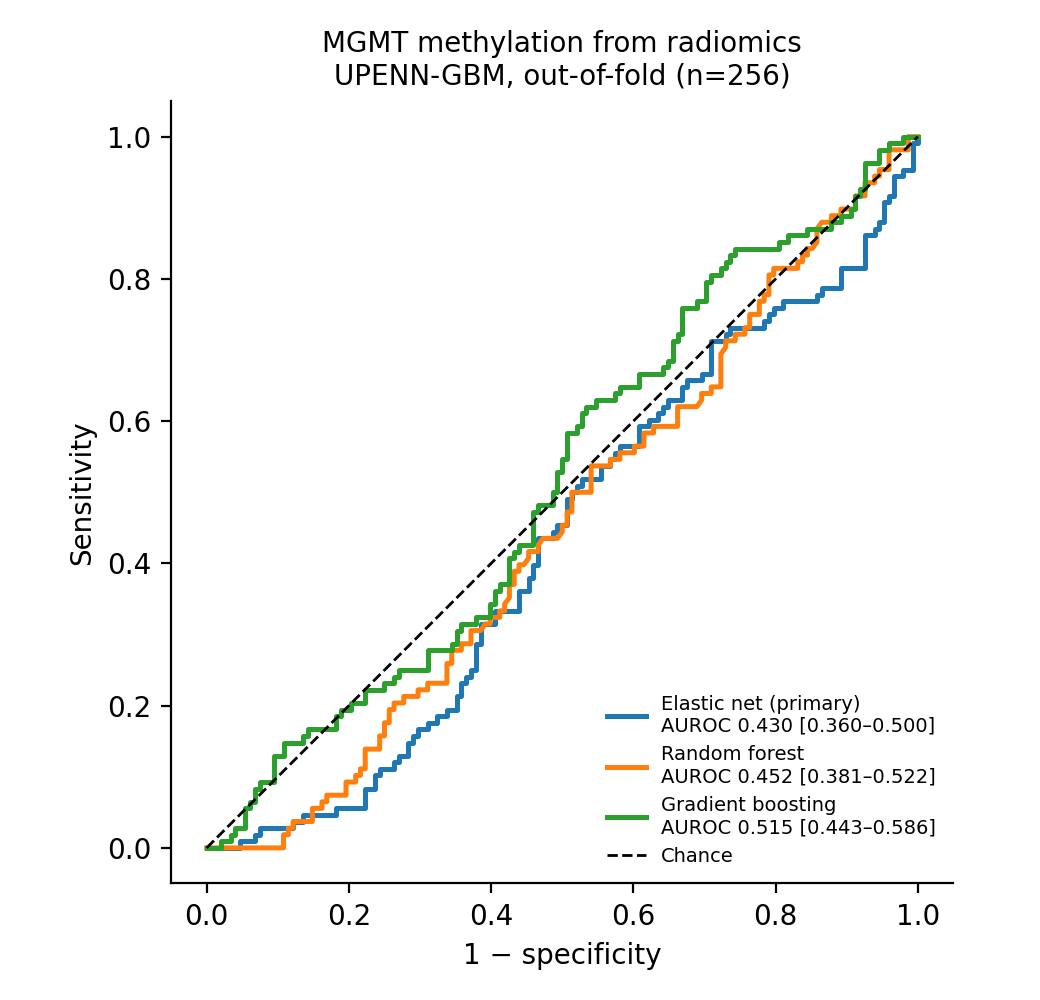
\includegraphics[width=0.62\textwidth]{fig1_roc.png}
\end{center}

\subsection*{Negative control}

Two hundred label permutations produced a null AUROC distribution centred on chance
(mean 0.498, 95\% interval 0.490--0.510). The observed value of 0.430 lies \emph{below}
that null, giving $p = 1.000$. This confirms two things: the pipeline contains no leakage
(a leaking pipeline shifts the null upward), and the observed performance is not merely
weak but indistinguishable from --- indeed slightly worse than --- random.

\begin{center}
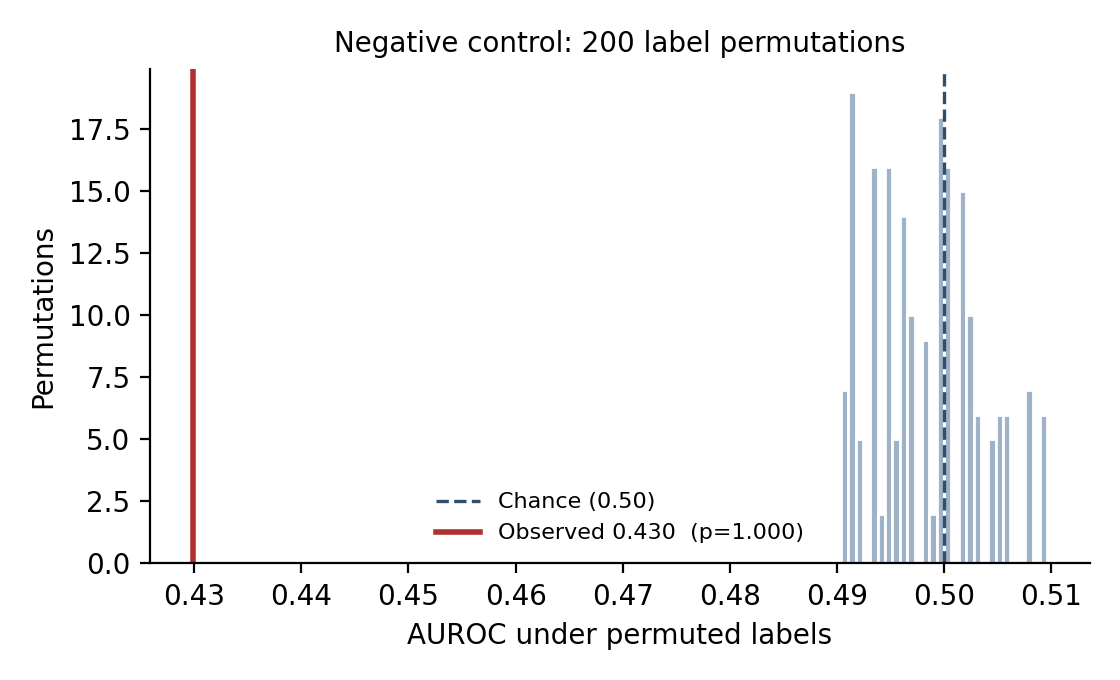
\includegraphics[width=0.78\textwidth]{fig2_permutation_null.png}
\end{center}

\section{Decision}

The plan specified: \emph{halt if the upper bound of the 95\% CI on internal AUROC is below
0.65.} The observed upper bound is \textbf{0.500}.

\textbf{Decision: STOP.} M2 (external validation) and M3 (deep learning and habitat
analysis) are not justified --- there is no signal to validate. No cloud compute was spent
on this milestone, and none is requested.

\section{Interpretation}

This agrees with the literature rather than contradicting it. The
RSNA-ASNR-MICCAI BraTS 2021 challenge was built on precisely this task and its organisers
concluded the signal may not be reliably learnable from imaging, with leading entries near
AUROC 0.6. Our result is a cleanly pre-registered, leakage-controlled replication of that
negative finding on an independent cohort.

\textbf{What this does exclude.} That handcrafted radiomic descriptors over automatic
segmentations of the four routine structural sequences carry recoverable MGMT information
in this cohort at this sample size.

\textbf{What this does not exclude.} A deep-learning model operating on voxels rather than
summary descriptors; features derived from perfusion or diffusion sequences (excluded here
for transferability); or manual rather than automatic segmentations. We regard the first as
substantially less likely given a null this flat across three model families, and we did
not test the third: only 59 patients have both manual-segmentation features and a definite
label, and running a 59-patient analysis after a null at n=256 would be noise-mining rather
than a sensitivity check.

\section{Recommendation for the glioma arm}

The wider difficulty is label availability, not modelling. Neither cohort in the revised
protocol carries a \textbf{glioma grade} label at all, and IDH is 19 positives of 630 in
development with no external label --- so the protocol's stated primary endpoint (grade) is
not computable, and IDH is not viable. MGMT was the only endpoint with labels in both
cohorts, and it is now tested and null.

We therefore recommend that the glioma arm be re-scoped around an endpoint that has
ground truth in an imaged cohort. The two candidates we can see:

\begin{enumerate}[leftmargin=1.6em,nosep]
\item \textbf{Overall survival} --- available for all 630 UPENN patients (644 deceased of
671 rows), and a genuine clinical question. No external survival data exists in our
holdings, so this would be internally validated only, which should be stated plainly.
\item \textbf{An imaged cohort spanning grades 2--4.} UT~Southwestern's 625 patients cover
the full grade range with IDH, 1p/19q and MGMT, but their images moved behind controlled
access during 2025. We hold the molecular labels and not the pixels. Obtaining the images
is a request, not a download.
\end{enumerate}

\noindent
We would value your view on whether either is worth pursuing, or whether the honest
conclusion is that this dataset combination cannot support the original question.

\section{How to verify this report}

Everything in \texttt{evidence/} is copied verbatim from an immutable run directory.

\begin{itemize}[leftmargin=1.4em,nosep]
\item \texttt{config.yaml} --- the plan as executed. Its SHA-256
(\texttt{0ec0a1df\ldots}) is recorded inside \texttt{results.json}; a plan altered
mid-analysis would not match.
\item \texttt{gates.json} --- eight integrity gates, each with expected value, observed
value and PASS/FAIL.
\item \texttt{oof\_*.csv} --- the out-of-fold predictions with labels, so every AUROC above
can be recomputed independently without rerunning anything.
\item \texttt{permutation\_null.json} --- all 200 null AUROC values.
\item \texttt{results.json}, \texttt{inputs.json} (input hashes), \texttt{env.txt}
(package versions), \texttt{MANIFEST.sha256}, \texttt{m1\_internal.py} (the code).
\item \texttt{gates\_FAILED\_first\_attempt.json} --- see below.
\end{itemize}

\subsection*{Two disclosures we would rather make than omit}

\textbf{A gate caught an error of ours before any model was fit.} The first attempt halted
at the cohort-size gate: expected 256, observed 262. The twelve feature files do not cover
identical subjects (enhancing tumour 604, oedema 611, necrotic core 602), and our planning
figure had been derived from a single file. Taking the union of subjects would have
median-imputed entire 144-feature blocks for four patients --- fabricating data. We
switched to complete cases across all twelve files, giving n=256, and documented the
superseded figure in the source. The failed run is retained rather than deleted, and its
gate record is included as \texttt{gates\_FAILED\_first\_attempt.json}.

\textbf{Determinism was tested, not assumed.} An independent re-run reproduced
byte-identical predictions, and a second full run performed after adding prediction output
reproduced all three AUROCs to twelve decimal places.

\vfill
\noindent{\color{qgrey}\rule{\textwidth}{0.4pt}}\\
{\footnotesize\color{qgrey}Run directory:
\texttt{paper-draft/02-revised-protocol-open-datasets/runs/20260806T223856Z-3f8bece}.
Data: UPENN-GBM, TCIA, CC BY 4.0 (Bakas et al., DOI 10.7937/TCIA.709X-DN49). No patient-level
data is reproduced in this report.}

\end{document}
